\begin{figure}[h]
	\centering
	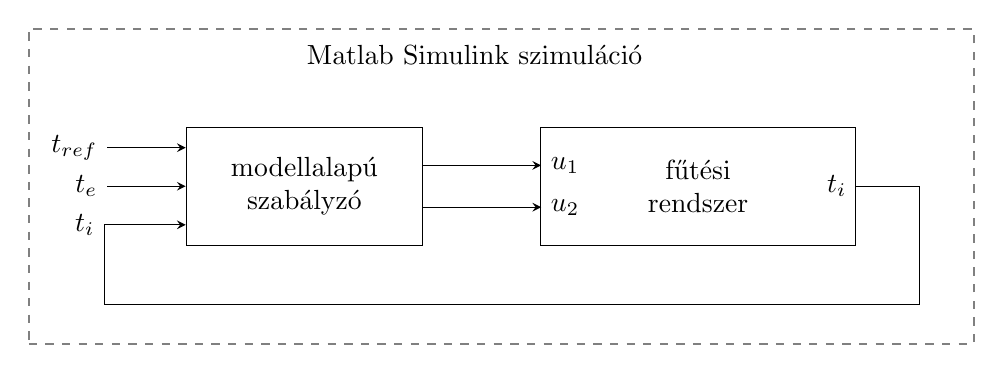
\begin{tikzpicture}[>=stealth,
	outer/.style={draw=gray,dashed,thick,inner sep=5pt}]

	% nagy blokkok
	\node[draw,rectangle, minimum height=1.5cm,minimum width=4cm] (plant) at (5,2.5) {\parbox{2cm}{\centering fűtési rendszer}};
	\node[draw,rectangle, minimum height=1.5cm,minimum width=3cm] (Control) at (0,2.5) {\parbox{2.5cm}{\centering modellalapú\\szabályzó}};
	
	% szaggatott vonal
	\node[draw,outer,rectangle, minimum height=4cm,minimum width=12cm,
	label={[label distance=-0.1cm, anchor=north]100:Matlab Simulink szimuláció}] (keret) at (2.5,2.5) {};
	
	
	% szabályzott mennyiségek
	\draw [->] (Control.10) node[right]{} -- +(15mm,0) node[right]{${u_{1}}$};
	\draw [->] (Control.350) node[right]{} -- +(15mm,0) node[right]{${u_{2}}$};
	
	%\draw[->] (Control.350) node[left]{} --  (plant.187) node[right]{${u_{2}}$};  %node[above left]{$\alpha_{radiator}$}; 
	%\draw[->] (Control.10) node[left]{} --  (plant.173) node[right]{${u_{1}}$} ;
	
	%\draw[->] (d.0) node[left]{heat [W]} ->  ++(3,0) ->  (house.180);
	
	
	% szabályzó bemenetei
	% a -| és |- máshogy fog törni, ha unconstraintelt.
	\draw [->] (plant.0)  node[left]{$t_i$} -|++(0.8,-1.5) -| ++(-9.25,0) |-  ++(-1.1,0) |- node[left]{$t_i$} (Control.198);
	
	%++(1.5cm,0) -- (2cm,0pt) -- (2.5cm,10pt);
	%\draw [->] (plant.0) node[left]{$t_i$ [\si{\celsius}]} -|++(1,0)|- -|++(-2.5,0)|- (Control.198) node[right]{}; %++(1.5cm,0) -- (2cm,0pt) -- (2.5cm,10pt);
	\draw [<-] (Control.180) node[right]{} -- +(-10mm,0) node[left]{$t_{e}$};
	\draw [<-] (Control.162) node[right]{} -- +(-10mm,0) node[left]{$t_{ref}$};
	
	%\draw[->] (House.180)  node[right]{${T_i}$} -| ++(-5.5,2)  |- (Control.180) ;
	%\draw[->] (d.20) -| ++(1,-1) |- (y.350);
	
	%\path 
	%(d.150)	 edge[<->] 	node[anchor=north,above]{valvePercent}	(y.270);
	
	\end{tikzpicture}

	\caption{A szimulációban szereplő elemek kapcsolata}
	\label{controlloop}
\end{figure}

%\begin{tikzpicture}[>=stealth,remember picture]
%\node[draw,rectangle,inner sep=0.5cm] (y) at (0,0) {$A$};
%\node[draw] (d) at (0,2) {%
%%	\begin{tikzpicture}[remember picture]
%%	\matrix [matrix of math nodes] (mat)
%%	{
%%		B & \phantom{C}   \\
%%		\phantom{B} & C \\
%%	};
%%	\end{tikzpicture}
%%};
%%\draw[->,shorten >= 6pt] (y.west) -| ++(-1,1) |- (mat-1-1);
%%\draw[->,shorten >= 6pt] (y.west) -| ++(-0.8,1) |- (mat-2-1);
%%\draw[->] ($(mat-2-2)+(14pt,0)$) -| ++(0.8,-1) |- (y.east);
%%\draw[->] ($(mat-1-2)+(14pt,0)$) -| ++(1,-1) |- (y.east);
%\end{tikzpicture}

